\subsection{Complete spatial profiles and compact summaries}\label{sec:anaheim}
The public Anaheim network has 416 nodes, 914 directed links and 1,406 positive OD demands \citep{tnfrc2024transportation}. Six largest demands change jointly from 0.8 to 1.2 times their published values; other demands remain fixed with endogenous route choices. Ten fixed free-flow shortest paths per OD exclude other zone centroids as intermediate nodes (first through node 39). This calculation uses the existing 41-state attribution columns.
To obtain interpretable region locations without requiring coordinates, define free-flow progress $p(v)=[d_s(v)-d_t(v)+d_s(t)]/[2d_s(t)]$, using shortest distances in the underlying undirected network with the smaller free-flow time on parallel roads. The origin has progress zero and destination progress one. Group tied levels, retain prefixes with two connected induced sides that separate the OD, and orient every region toward the origin. This distance-based family depends on the network and query, before inspecting any attribution. It is a prescribed family, not all connected regions.

The case asks one transport question: how does the signed crossing-cost
response of the demand change evolve along the origin--destination
direction, and does the variation come mainly from the study traffic's
congestion adjustment or from background rerouting?
Figure~\ref{fig:anaheimprofile} gives the answer for the query with the
largest early--late difference: the account as a function of progress
over the complete family, with the three prespecified positions marked,
and the four-part same-state decomposition along the same axis. The
profiles of the remaining five queries stay positive with family ranges
spanning roughly one to one and a half orders of magnitude
(largest-to-smallest account ratios 12.5--36.9); the complete per-query
numbers --- system contributions, unrestricted and family ranges,
region counts and the accounts of the three prespecified positions ---
are collected in Appendix~\ref{app:anaheimsettings}
(Table~\ref{tab:anaheim}), with the early--late mechanism differences
in Table~\ref{tab:anaheimmechanism}.
\begin{figure}[t]\centering
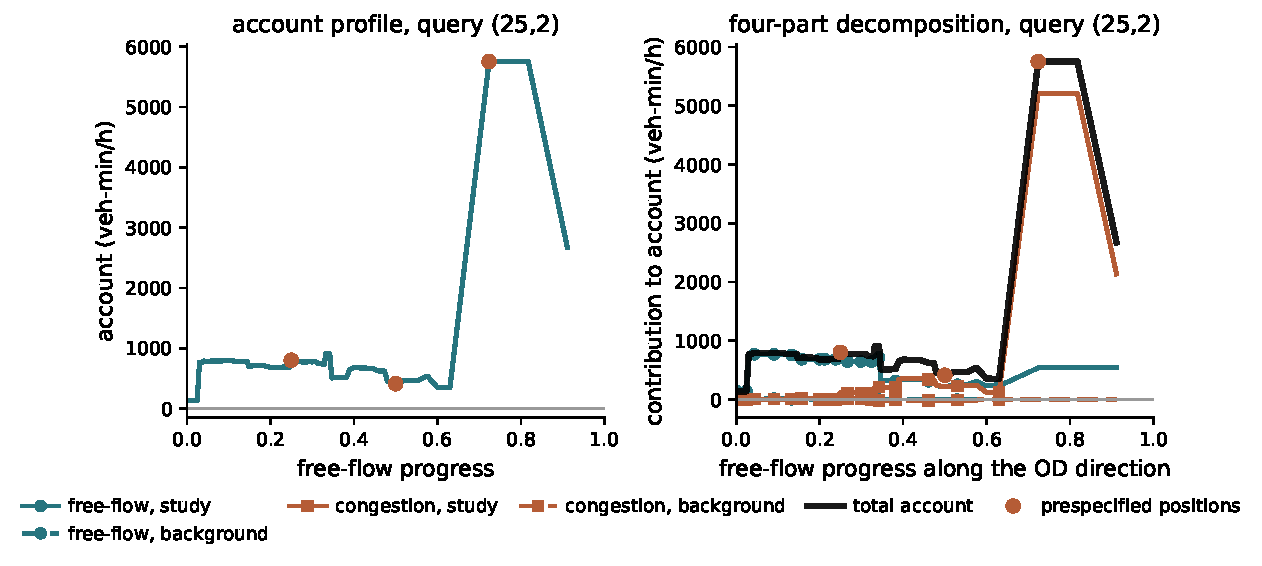
\includegraphics[width=0.99\linewidth]{../figures/fig_v107_anaheim_profile.pdf}
\caption{Anaheim spatial response profile for query $(25,2)$ over the
distance-based family. Left: the account versus free-flow progress
along its own OD direction; ochre dots mark the three prespecified
positions (nearest admissible gaps to progress $0.25$, $0.50$,
$0.75$). Right: the four-part same-state decomposition, crossing
free-flow and congestion weights with study and background responses
at identical states (teal: free-flow weights, ochre: congestion
weights; solid: study response, dashed: background); the grey curve is
the total account. Components close within $2\times10^{-12}$
vehicle-minutes per hour.}\label{fig:anaheimprofile}
\end{figure}
Query $(25,2)$ falls from 801.5 at progress $0.250$ to 412.0 at $0.500$
and then rises to the family maximum 5751.2, which holds on the plateau
from progress $0.724$ to $0.818$ before falling back to 2673.1 at
$0.911$. The decomposition panel locates the mechanism. At the early
position the account is dominated by the free-flow study response
($669.3$ of the total $801.5$, congestion study $111.5$, background
below $11$); at the middle position the two study terms are comparable
($211.5$ free-flow against $212.6$ congestion of the total $412.0$,
background below $11$); at the late position the congestion study term
reaches $5213.7$ while both background terms are below $0.1$ in
absolute value: the rise is congestion adjustment of the study traffic
itself on destination-side links, not background rerouting. The
decomposition is additive at a common equilibrium state and identifies
the contribution of each response--weight component.

Because this family is totally ordered by progress, it also supports
piecewise common summaries. The construction is stated for any ordered
family.
\begin{proposition}[minimal contiguous boundary summary]\label{prop:segmented}
Fix an ordered family of boundary accounts $a_1,\ldots,a_N$ and a
tolerance $\epsilon>0$. Among partitions into contiguous intervals
whose every interval has range at most $2\epsilon$ and does not
strictly mix signs, the longest-feasible-prefix procedure returns one
with the minimum number of intervals.
\end{proposition}
\begin{proof}
No feasible first interval can extend past the longest feasible prefix,
so every optimal partition starts with a prefix no longer than the
greedy choice; replacing the first interval of an optimal partition by
the full greedy prefix cannot make the remainder infeasible, and the
same argument applies inductively to the remainder.
\end{proof}
Its value here is the coupling to the boundary scan, the
node-difference interpretation, and a stated tolerance: a single
interval reproduces the common summary of Eq.~\eqref{eq:familycommon}.
On Anaheim, ordering by native progress, the 83--211 accounts per query
reduce to 4--14 segments at the $5\%$ tolerance (compression
$90.4$--$95.2\%$), each within the stated tolerance by construction;
the tolerance frontier is reported alongside the Sioux Falls results
in Figure~\ref{fig:commonsummary}. On Sioux Falls the mixed-direction
family ordered by free-flow progress compresses less --- the median
query needs 38 segments for 86.5 regions --- because distinct
directions at nearby positions carry genuinely different accounts.
Neither construction changes any original account; both summarize the
same computed accounts with a stated worst error. Aggregation timings
and the original construction costs appear in
Appendix~\ref{supp:timing}.
